% Phase 2 results chapter — TUM M.Sc. Data & Society (English).
% Standalone KOMA-Script article so the file compiles without the full TUM
% thesis class. Sectioning matches a thesis results chapter, not a CIKM reprint.
%
% Compile: pdflatex main && biber main && pdflatex main && pdflatex main
%
% Figures: copies of thesisExperiment/results_phase2/figures/ (and
% analysis_phase2/figures/). If a later analysis_full pass produces replacement
% panels, swap the files in figures/ and keep the caption numbers.
%
% Isolation: this folder does not write Phase 1 runs/ or results/tables/.
% Do not commit .env.

\documentclass[
  11pt,
  a4paper,
  oneside,
  bibliography=totoc,
  listof=totoc,
  captions=tableheading,
  headings=normal,
  numbers=noenddot
]{scrartcl}

\usepackage[T1]{fontenc}
\usepackage[utf8]{inputenc}
\usepackage{lmodern}
\usepackage[english]{babel}
% TUM skill §11 specifies English quotation punctuation, not German „quotes“.
% csquotes \enquote{...} is the TUM-safe wrapper; babel english selects “...”.
\usepackage[autostyle,english=american]{csquotes}
\usepackage{microtype}
\usepackage[margin=2.5cm]{geometry}
\usepackage{setspace}
\onehalfspacing
\emergencystretch=2em
\usepackage{graphicx}
\usepackage{array}
\usepackage{booktabs}
\usepackage{tabularx}
\usepackage{tabulary}
\usepackage{longtable}
\usepackage{multirow}
\usepackage{makecell}
\usepackage{threeparttable}
\usepackage{xcolor}
\usepackage{tikz}
\usetikzlibrary{arrows.meta,positioning,fit,calc}
\usepackage{caption}
\usepackage{subcaption}
\usepackage{enumitem}
\usepackage{amsmath,amssymb}
\usepackage[style=authoryear,
            backend=biber,
            maxcitenames=3,
            mincitenames=1,
            maxbibnames=99,
            giveninits=true,
            uniquename=init,
            uniquelist=false,
            doi=true,
            url=false,
            isbn=false,
            dashed=false,
            natbib=true]{biblatex}
\addbibresource{references.bib}
\usepackage[hidelinks]{hyperref}
\usepackage{xurl}
\usepackage[nameinlink,capitalize,noabbrev]{cleveref}

\captionsetup{
  format=plain,
  labelfont={bf,small},
  font=small,
  skip=6pt,
  justification=RaggedRight,
  singlelinecheck=false
}
\captionsetup[table]{position=top,skip=4pt}
\captionsetup[figure]{position=bottom,skip=6pt}

\setkomafont{disposition}{\rmfamily\bfseries}
\setkomafont{title}{\rmfamily\bfseries}
\newcommand{\MPR}{\textsc{mpr}}
\newcommand{\MI}{\textsc{mi}}
\newcommand{\kstar}{$k^{\ast}$}
\newcommand{\ie}{\textit{i.e.}}
\newcommand{\eg}{\textit{e.g.}}
\newcommand{\cf}{\textit{cf.}}

\title{Phase 2 Results:\\
Topology, Identity Mix, and Scoring Mode\\
in a Climate-Firestorm Simulation}
\author{TUM M.Sc.\ Data and Society --- thesis results chapter (standalone)}
\date{Harvest stamp: 19 September 2026}

\begin{document}
\maketitle

\begin{abstract}
This chapter reports the Phase~2 campaign of the climate-firestorm simulation.
The campaign crossed eight network topologies with homogeneous (H) and heterogeneous (He) identity mixes and with two auditor instruments, then compared a reconstructed Debnath hashtag graph against a custom-graph (D-net) simulation.
Discrete \MPR{} (dual-run headline) and continuous \MPR{} (continuous-only headline) are different instruments; this chapter never averages them.
The harvest is a real \texttt{gpt-4o-mini} run with $N=1$, eight hops, and \texttt{thesisGrade=false}.
Hatched dead cells remain in the grid.
The Debnath comparison is structural: 814k tweet identifiers were not hydrated, and Debnath's skip-gram window of eight is not this protocol's hop budget.
\end{abstract}

\tableofcontents
\listoffigures
\listoftables
\clearpage

\section{Purpose of this chapter}
\label{sec:intro}

This chapter reports the Phase~2 results of the climate-firestorm simulation.
The purpose is to describe, under documented limits, how eight network topologies, homogeneous versus heterogeneous identity mixes, and two auditor instruments move misinformation scores on six geoengineering articles.
The chapter is a thesis-style results account.
It is not a reprint of the CIKM linear-chain study on commercial and crime news \parencite{maurya2025simulating}, and it is not a Twitter digital twin of Debnath and colleagues' 814,924-tweet observational map \parencite{debnath2023conspiracy}.

The theoretical spine remains online firestorms as defined by \textcite{pfeffer2014firestorms}: a sudden discharge of large quantities of negative word-of-mouth in social media, often with high affective charge.
Their Outlook section lists \emph{seven} interrelated factors, not six.
Section~\ref{sec:dnet} restates those seven factors from the Debnath-versus-D-net mapping and records the thesis six-knob list as a computational remapping.
Cross-media dynamics has no engine knob and is held.

Phase~2 asked a narrower empirical question than a full Pfeffer confirmation.
Holding surprise as a drip seed and holding the clock at eight ticks, do topology, identity mix, and auditor mode change live-cell mean \MI{} on climate seeds?
The harvest answers that question only descriptively.
\texttt{summary.json} sets \texttt{thesisGrade} to false.
$N=1$ with graph seed 42 forbids error bars and replicate inference.

The remainder of the chapter follows a single path.
Section~\ref{sec:methods} snapshots the protocol.
Section~\ref{sec:instruments} separates discrete from continuous \MPR{}.
Section~\ref{sec:topology} reports all eight topologies.
Section~\ref{sec:hhe} reports personas and mixes without averaging the two instruments.
Section~\ref{sec:designs} reports the five numbered comparisons from the full analysis (C1--C5).
Section~\ref{sec:pooled} states that cell pooling concatenates rows and is not a physical super-graph.
Section~\ref{sec:dnet} compares D-net structure and Pfeffer observables with the Debnath hashtag fallback.
Section~\ref{sec:limits} states limitations.
Section~\ref{sec:conclusion} closes.

Figures are copies of \path{thesisExperiment/analysis_full/figures/} (\texttt{fig00}--\texttt{fig22}).
Comparison panels follow \texttt{COMPARISONS.md}.
Exploratory rank tests in that file are not treated as replicate inference.

\section{Methods snapshot}
\label{sec:methods}

The Phase~2 campaign reused the existing CIKM engine entry point (\texttt{node index.js --config}) with thesis-layer configs under \texttt{thesisExperiment/configs/phase2/}.
Each node is a persona-conditioned \texttt{gpt-4o-mini} agent.
Allowed actions are forward, reinterpret, and drop.
Propagation runs first; the auditor scores rewrites in a second pass \parencite{maurya2025simulating}.
The auditor is also \texttt{gpt-4o-mini}, so the scores are LLM-as-judge values in the sense of \textcite{zheng2023judge}, not human ratings.

\Cref{fig:methods} sketches the two-phase pipeline.
A ground-truth article enters at the drip seed.
Persona-conditioned nodes rewrite or forward the text along the graph.
The auditor returns an event \MI{} on five yes/no items.
Discrete \MI{} equals the count of missing plus incorrect answers and therefore sits in $\{0,1,2,3,4,5\}$.
Continuous \MI{} is a float on approximately the same $0$--$5$ range.
Node \MPR{} is the mean of scored event \MI{} for that node and article.
The cell headline used below is parser \texttt{meanMI} (mean scored-event \MI{} on live cells with \texttt{nScored}$>1$).
\texttt{meanNodeMPR} is the mean of node means of the same headline.
The two scalars sit beside each other; they are not mixed into one number.

\begin{figure}[t]
\centering
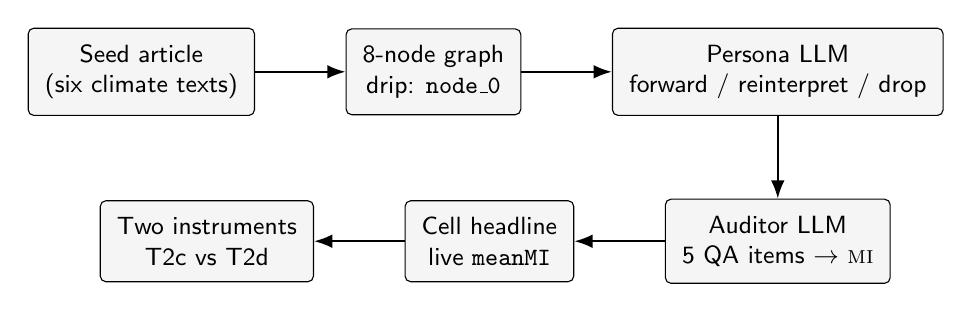
\begin{tikzpicture}[
  font=\small\sffamily,
  box/.style={draw, rounded corners=2pt, align=center, inner sep=6pt, fill=black!4},
  arr/.style={-{Latex}, thick}
]
\node[box] (seed) {Seed article\\(six climate texts)};
\node[box, right=1.15cm of seed] (graph) {8-node graph\\drip: \texttt{node\_0}};
\node[box, right=1.15cm of graph] (agent) {Persona LLM\\forward / reinterpret / drop};
\node[box, below=1.05cm of agent] (aud) {Auditor LLM\\5 QA items $\to$ \MI{}};
\node[box, left=1.15cm of aud] (agg) {Cell headline\\live \texttt{meanMI}};
\node[box, left=1.15cm of agg] (split) {Two instruments\\T2c vs T2d};
\draw[arr] (seed) -- (graph);
\draw[arr] (graph) -- (agent);
\draw[arr] (agent) -- (aud);
\draw[arr] (aud) -- (agg);
\draw[arr] (agg) -- (split);
\end{tikzpicture}
\caption[Methods schematic for Phase~2]{Methods schematic for Phase~2.
A ground-truth climate article is rewritten by persona-conditioned \texttt{gpt-4o-mini} nodes on an eight-node graph, then scored by a five-item auditor.
Discrete and continuous campaigns are separate configs.
Network \kstar{} is the first irreversible crossing of mean \MI{}$>3$, censored at eight ticks.
This drawing is a protocol snapshot, not an empirical result.}
\label{fig:methods}
\end{figure}

\subsection{Grid that was harvested}

Phase~2 isolated its outputs from Phase~1.
Runs live under \texttt{thesisExperiment/runs\_phase2/}; tables live under \texttt{thesisExperiment/results\_phase2/}.
The discrete $12\times 12$ Phase~1 campaign in \texttt{runs/} and \texttt{results/tables/} was not overwritten and is not spliced into the headlines below.

\Cref{tab:grid} records the harvested grid.
T2c denotes continuous-only scoring.
T2d denotes dual scoring, whose \emph{headline} is discrete.
Homogeneous (H) cells cycle one of twelve personas on eight nodes.
Heterogeneous (He) cells cycle one of six mixes of eight persona identifiers.
Six core articles run sequentially in each config: SCoPEx 2017, chemtrails--Gates 2018--2021, SAI geoengineering, the Paris Agreement, climate consensus, and polar bears.
The expected thesis grid is $1{,}728$ cells.
The harvest reports $0$ missing cells.

\begin{table}[t]
\centering
\caption[Phase~2 harvest grid]{Phase~2 harvest grid.
Source: \texttt{results\_phase2/summary.json} (stamp 2026-09-19T05:27:59.674Z).
Dead cells are hatched after real LLM calls (\texttt{nScored}$\le 1$, \texttt{llmCalls}$>0$) and are excluded from live means.}
\label{tab:grid}
\begin{threeparttable}
\small
\begin{tabular}{lrrrr}
\toprule
Slice & Configs & Cells & Hatched dead & Status \\
\midrule
T2c\_H (cont., homo.) & 96/96 & 576/576 & 94 & complete \\
T2d\_H (dual-disc., homo.) & 96/96 & 576/576 & 98 & complete \\
T2c\_He (cont., hetero.) & 48/48 & 288/288 & 50 & complete \\
T2d\_He (dual-disc., hetero.) & 48/48 & 288/288 & 48 & complete \\
D-net custom graph & 4 configs & 8 article-rows & 0 & complete \\
\midrule
Thesis grid (T2 only) & 288 & 1,728 & 290 & \texttt{thesisGrade} false \\
\bottomrule
\end{tabular}
\begin{tablenotes}[para,flushleft]
\footnotesize
An earlier parse note counted 292 hatched rows; the official harvest tables use 290.
This chapter uses 290.
\end{tablenotes}
\end{threeparttable}
\end{table}

\subsection{Shared protocol}

Every T2 cell used eight nodes, eight ticks, eight hops, inbox cap~4, trust threshold $0.15$, action weights $0.35$/$0.50$/$0.15$ (forward/reinterpret/drop), relation evolution on (\texttt{trustDelta}$=0.05$), activity pattern \texttt{always}, and \texttt{graphRandomSeed: 42}.
The seed is always \texttt{node\_0} (drip).
The model is \texttt{gpt-4o-mini} for agent and auditor.
Replicates: $N=1$.

Eight hops is a logged cost cut versus the CIKM chain length of 30 \parencite{maurya2025simulating}.
It is not Debnath's hop protocol.
Debnath and colleagues define a skip-gram \emph{context window of eight words} inside a tweet when they estimate $p_{\mathrm{together}}$ with \enquote{chemtrails} \parencite{debnath2023conspiracy}.
That window is a word-embedding hyperparameter.
It is not this campaign's tick budget.
The public R codes use an $n=10$ n-gram implementation detail \parencite{geoeng2023codes}; the paper text says eight.

\subsection{Topologies and identity}

The eight generators are \texttt{linear\_chain}, \texttt{ring}, \texttt{random\_er} \parencite{erdos1960evolution}, \texttt{small\_world} \parencite{watts1998collective}, \texttt{scale\_free} \parencite{barabasi1999emergence}, \texttt{echo\_chamber}, \texttt{polarized}, and \texttt{hierarchical}.
Linear chain is the CIKM object \parencite{maurya2025simulating}.
It is included so the climate corpus can be read against that topology, not because a chain is a firestorm clustering contrast.
Scale-free uses Barabási--Albert $m=2$.
ER uses $p=0.42$ with \texttt{minSeedOutDegree=2} so the drip seed cannot have out-degree zero.

Twelve homogeneous personas fall into three families: conspiracy (four), climate action (three), and science/environment (five).
Belief profiles are theory-faithful reductions of Debnath discourse types, not HDBSCAN centroids on 814k tweets \parencite{debnath2023conspiracy}.
Six heterogeneous mixes vary conspiracy share from four of eight (\texttt{mix\_00}) to zero of eight (\texttt{mix\_02}).
\texttt{mix\_02} is the expert-inclusive mix: climate-action, science, and environment identifiers only.

\subsection{Pfeffer knobs: swept, held, measured}

\textcite{pfeffer2014firestorms} do not name valence, surprise, identity, clustering, echo, and temporal acceleration as a canonical six-factor theory.
The campaign treats those six names as engine knobs.
Valence is varied by the six articles and by persona tone.
Identity alignment is swept (H versus He).
Network clustering is swept (eight topologies).
Information echo is measured (homophily on the last-tick graph) and additionally wired in the echo-chamber and polarised generators.
Surprise is held as drip seeding.
Temporal acceleration is held at eight ticks.
Cross-media dynamics, the sixth Outlook factor in 2014, has no broadcast agent and is held.

\subsection{Dead cells and \texorpdfstring{\kstar{}}{k*}}

A cell is hatched dead when \texttt{nScored}$\le 1$ after real LLM calls.
Dead cells are kept.
They are not imputed as \MI{}$=0$ and they are not read as \enquote{mix immunises}.
Live means drop those cells and report \texttt{n\_live}.

Network \kstar{} is the first tick at which network-mean \MI{}$>3$ (propaganda) and mean \MI{} stays $>3$ on every later tick with data.
If the series later returns to $\le 3$, \kstar{} is undefined (none), not zero.
The crossing is right-censored at eight ticks, so irreversibility is weak.
Dual \kstar{} uses the discrete series.
Continuous \kstar{} uses the continuous series.
The two rates are not added.

Independent-cascade models treat adoption as a binary infection \parencite{kempe2003influence}.
This engine carries mutating text plus an auditor, so \kstar{} clocks semantic degradation rather than a binary infected bit.
The clock is still a simulation artefact on eight ticks, not an empirical firestorm duration.

\section{Two scoring instruments}
\label{sec:instruments}

Phase~2 ran two auditor modes as separate campaigns.
Continuous configs (prefix T2c) set \texttt{miScoringMode} to continuous.
The headline \MI{}/\MPR{} is the continuous auditor float.
Dual configs (prefix T2d) call both a discrete auditor and a continuous sidecar on the same events.
The dual \emph{headline} is the discrete $0$--$5$ score.
The sidecar continuous value is a scoring diagnostic.
Dual gap (discrete minus sidecar continuous) is not a third ground-truth \MPR{}.

These two headlines are not the same quantity.
Dual-discrete H ($1.6814$) is not \enquote{the same \MPR{} as continuous H ($0.8643$) but higher}.
The auditors are different instruments.
Dual-discrete sits higher than continuous on every topology in this harvest.
That pattern is a scoring-mode effect.
It is not evidence that the discrete campaign found more misinformation in a shared unit.

\Cref{tab:headlines} reports live-cell means of \texttt{meanMI}.
Dead cells are excluded.
H and He remain separate.
The harvest cross-check on H matches the recomputed live means to four decimals.

\begin{table}[t]
\centering
\caption{Live-cell headline \MPR{} by arm and instrument.
Dead cells excluded.
$N=1$.
Do not pool the two columns or the two rows.}
\label{tab:headlines}
\begin{threeparttable}
\small
\begin{tabular}{lrrrr}
\toprule
Arm & Cont.\ \MPR{} (T2c) & $n$ live cont. & Dual-disc.\ \MPR{} (T2d) & $n$ live dual \\
\midrule
H (homogeneous) & 0.8643 & 480 & 1.6814 & 478 \\
He (heterogeneous) & 1.0192 & 238 & 2.0800 & 240 \\
\midrule
He $-$ H (same mode only) & 0.1549 & --- & 0.3986 & --- \\
Mean dual gap (sidecar) & --- & --- & 0.8804 (H) / 1.1145 (He) & --- \\
\bottomrule
\end{tabular}
\end{threeparttable}
\end{table}

The same cells as \texttt{meanNodeMPR} (not interchangeable with \texttt{meanMI}) are H continuous $0.8630$, H dual $1.6839$, He continuous $1.0140$, He dual $2.0737$.
This chapter leads with \texttt{meanMI} and treats \texttt{meanNodeMPR} as a sidecar of the same instrument.

\Cref{fig:dualgap} plots dual gap and agreement.
The gap is large on both arms.
Using it as an \MPR{} would smuggle the discrete--continuous disagreement into a third league table.
The figure is a diagnostic only.

\begin{figure}[t]
\centering
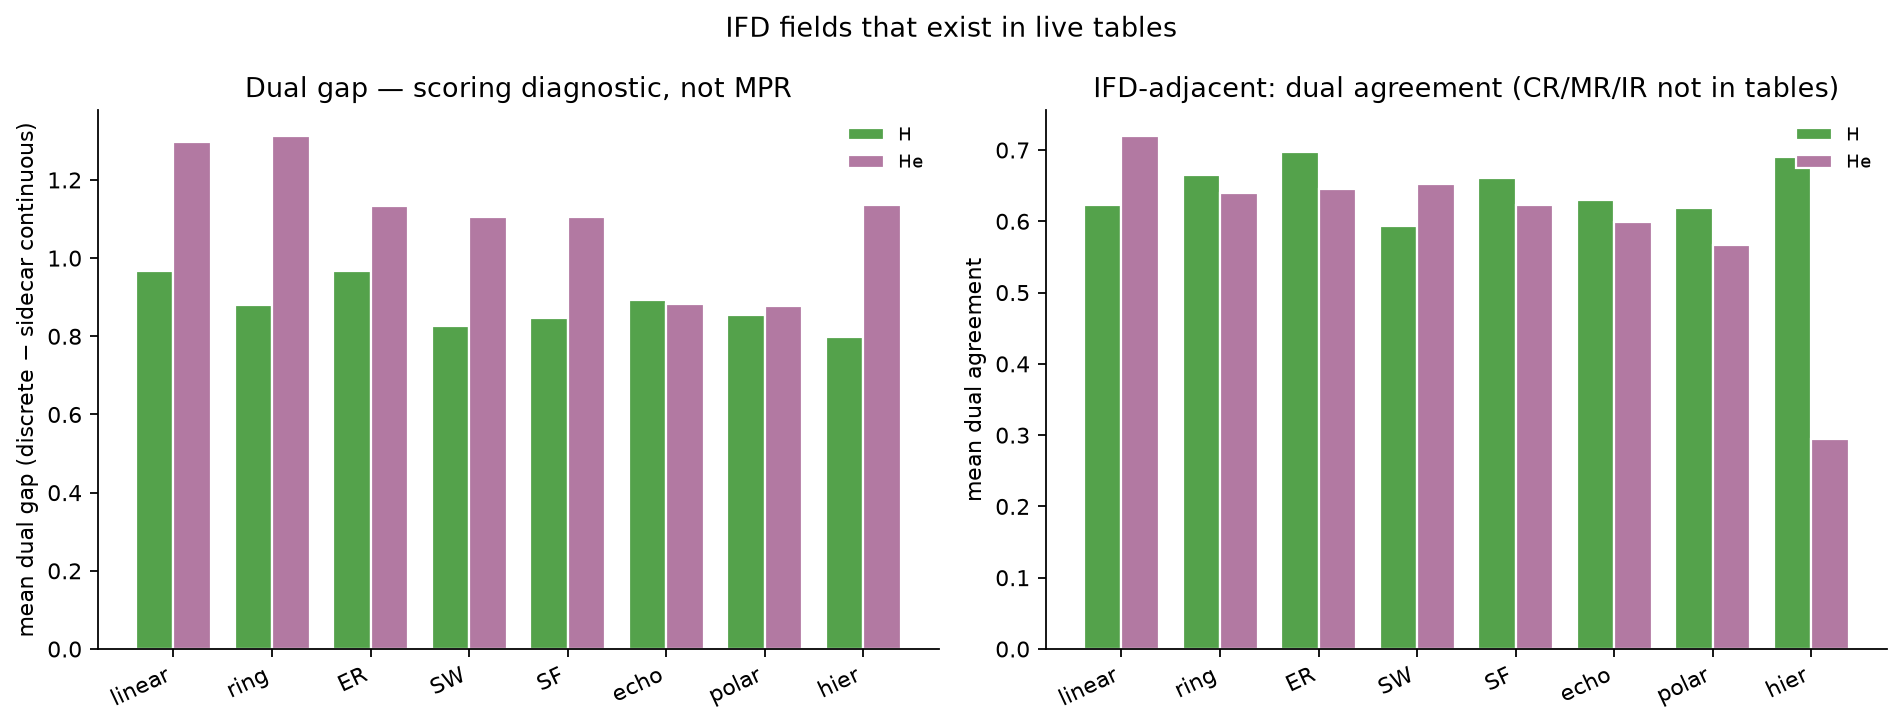
\includegraphics[width=\textwidth]{figures/fig20_ifd_dual_gap_agreement.png}
\caption[Dual gap and agreement]{Dual gap (discrete headline minus sidecar continuous) and dual agreement.
The gap is a scoring diagnostic, not a ground-truth \MPR{}.
$N=1$, eight hops.
Source: \texttt{fig20\_ifd\_dual\_gap\_agreement.png}.}
\label{fig:dualgap}
\end{figure}

\section{All eight topologies}
\label{sec:topology}

Topology is the clustering knob in the remapping of \textcite{pfeffer2014firestorms}.
Phase~2 swept eight generators rather than the Phase~1 pair (scale-free versus ER).
\Cref{fig:topo} shows live-cell mean \texttt{meanMI} for each generator, with discrete and continuous bars side by side and H and He in separate panels.
Rank order is not the same across scoring modes.
A single \enquote{best topology} from a pooled number is not available from this harvest.

\begin{figure}[t]
\centering

\includegraphics[width=\textwidth]{figures/fig01_topology_mpr_discrete_vs_continuous.png}
\caption{Live-cell mean \texttt{meanMI} by topology, scoring mode, and arm.
Left: homogeneous.
Right: heterogeneous.
Discrete (T2d) and continuous (T2c) bars are not averaged.
Dashed line in later figures marks the propaganda threshold \MI{}$=3$; this panel uses the raw $0$--$5$ scale.
$N=1$.
Source: \texttt{fig01\_topology\_mpr\_discrete\_vs\_continuous.png}.}
\label{fig:topo}
\end{figure}

\Cref{tab:topoH,tab:topoHe} list the same means with live counts, \kstar{} rates, and dead rates.
Linear chain and ring are short, low-degree paths.
Hierarchical is a different degree sequence.
With $N=1$ the gaps are descriptive.
They are not a significance claim about ER versus scale-free.

\begin{table}[p]
\centering
\caption{Homogeneous (H) topology headlines.
Each topology has 72 cells per mode (12 personas $\times$ 6 articles).
Live means exclude hatched dead cells.}
\label{tab:topoH}
\scriptsize
\begin{tabular}{lrrrrrrrr}
\toprule
Topology & $n$ live dual & Disc.\ \MPR{} & \kstar{} dual & Dead dual & $n$ live cont. & Cont.\ \MPR{} & \kstar{} cont. & Dead cont. \\
\midrule
linear chain & 68/72 & 1.6127 & 14.7\% & 5.6\% & 62/72 & 0.9129 & 14.5\% & 13.9\% \\
ring & 61/72 & 1.6402 & 18.0\% & 15.3\% & 65/72 & 0.9160 & 15.4\% & 9.7\% \\
random ER & 56/72 & 1.7809 & 19.6\% & 22.2\% & 57/72 & 0.8736 & 14.0\% & 20.8\% \\
small world & 59/72 & 1.5977 & 20.3\% & 18.1\% & 56/72 & 0.7215 & 12.5\% & 22.2\% \\
scale-free & 57/72 & 1.7034 & 21.1\% & 20.8\% & 60/72 & 0.9205 & 16.7\% & 16.7\% \\
echo chamber & 61/72 & 1.7984 & 23.0\% & 15.3\% & 65/72 & 0.8233 & 12.3\% & 9.7\% \\
polarised & 57/72 & 1.7005 & 21.1\% & 20.8\% & 65/72 & 0.8356 & 15.4\% & 9.7\% \\
hierarchical & 59/72 & 1.6315 & 23.7\% & 18.1\% & 52/72 & 0.8751 & 11.5\% & 27.8\% \\
\bottomrule
\end{tabular}
\end{table}

\begin{table}[p]
\centering
\caption{Heterogeneous (He) topology headlines.
Each topology has 36 cells per mode (6 mixes $\times$ 6 articles).}
\label{tab:topoHe}
\scriptsize
\begin{tabular}{lrrrrrrrr}
\toprule
Topology & $n$ live dual & Disc.\ \MPR{} & \kstar{} dual & Dead dual & $n$ live cont. & Cont.\ \MPR{} & \kstar{} cont. & Dead cont. \\
\midrule
linear chain & 33/36 & 2.0852 & 24.2\% & 8.3\% & 32/36 & 0.8638 & 0.0\% & 11.1\% \\
ring & 33/36 & 2.1768 & 39.4\% & 8.3\% & 33/36 & 0.8760 & 3.0\% & 8.3\% \\
random ER & 29/36 & 2.0412 & 27.6\% & 19.4\% & 29/36 & 0.6593 & 0.0\% & 19.4\% \\
small world & 32/36 & 1.9096 & 28.1\% & 11.1\% & 31/36 & 0.7545 & 3.2\% & 13.9\% \\
scale-free & 29/36 & 1.9924 & 31.0\% & 19.4\% & 30/36 & 0.8157 & 6.7\% & 16.7\% \\
echo chamber & 30/36 & 1.9632 & 23.3\% & 16.7\% & 32/36 & 1.3775 & 9.4\% & 11.1\% \\
polarised & 26/36 & 1.8830 & 42.3\% & 27.8\% & 25/36 & 1.4137 & 12.0\% & 30.6\% \\
hierarchical & 28/36 & 2.5934 & 42.9\% & 22.2\% & 26/36 & 1.5242 & 30.8\% & 27.8\% \\
\bottomrule
\end{tabular}
\end{table}

On homogeneous continuous cells, scale-free is highest ($0.9205$) and small-world is lowest ($0.7215$).
On homogeneous dual-discrete cells, echo chamber is highest ($1.7984$) and small-world is lowest ($1.5977$).
On heterogeneous continuous cells, hierarchical is highest ($1.5242$) and ER is lowest ($0.6593$).
On heterogeneous dual-discrete cells, hierarchical is highest ($2.5934$) and polarised is lowest ($1.8830$).

Hierarchical and polarised He cells also show high dead rates (about 28--31\% continuous).
A live-only mean on a half-dead topology inflates uncertainty.
Those rows describe the surviving cascades, not a clean generator effect.

\Cref{fig:kstar} reports \kstar{} occurrence on live cells.
He dual-discrete \kstar{} rates sit well above He continuous rates (32.1\% versus 7.6\% collapsed).
The discrete instrument crosses and stays above $3$ more often in this harvest.
That is still a scoring-mode fact, not a second firestorm clock on a shared unit.

\begin{figure}[t]
\centering

\includegraphics[width=\textwidth]{figures/fig09_kstar_rates.png}
\caption{Share of live cells with irreversible network \kstar{} (mean \MI{}$>3$ with no later recovery), by topology and scoring mode.
Dual \kstar{} uses the discrete series; continuous \kstar{} uses the continuous series.
The two rates are not added.
Right-censored at eight ticks.
$N=1$.
Source: \texttt{fig09\_kstar\_rates.png}.}
\label{fig:kstar}
\end{figure}

\Cref{fig:dead} shows hatched dead-cell rates.
Overall, 290 of 1,728 thesis cells (16.8\%) are hatched after LLM.
Hierarchical H continuous is 27.8\% dead; polarised He continuous is 30.6\% dead.
Those generators contribute fewer scored events.
The hatch pattern is part of the result, not a footnote.

\begin{figure}[t]
\centering

\includegraphics[width=\textwidth]{figures/fig08_dead_cell_rates.png}
\caption{Hatched dead-cell rate by topology, arm, and scoring mode.
Dead means \texttt{nScored}$\le 1$ after real LLM calls.
Hatched cells are kept and are not scored as mix immunity.
$N=1$.
Source: \texttt{fig08\_dead\_cell\_rates.png}.}
\label{fig:dead}
\end{figure}

\section{Homogeneous versus heterogeneous identity}
\label{sec:hhe}

Identity alignment is the remapping of Pfeffer factor~5 (lack of diversity) into a persona mix \parencite{pfeffer2014firestorms}.
H cells use one persona on all eight nodes.
He cells use a documented eight-identifier mix.
\Cref{fig:hhe} plots collapsed live-cell means for each instrument.

\begin{figure}[t]
\centering

\includegraphics[width=0.92\textwidth]{figures/fig02_h_vs_he_mpr.png}
\caption{Collapsed live-cell \texttt{meanMI} for homogeneous (H) versus heterogeneous (He) arms, separately for continuous (T2c) and dual-discrete (T2d) headlines.
The two panels are not averaged.
$N=1$.
Source: \texttt{fig02\_h\_vs\_he\_mpr.png}.}
\label{fig:hhe}
\end{figure}

Collapsed He is higher than collapsed H on both instruments (continuous $+0.1584$; dual-discrete $+0.3986$).
That ordering is the opposite of a pooled \enquote{hetero buffers firestorms} claim of the sort associated with mixed CIKM chains \parencite{maurya2025simulating}.
The H mean mixes conspiracy personas (continuous about $2$--$2.5$) with scientists (continuous near $0$).
The He mean mixes conspiracy-heavy \texttt{mix\_00}/\texttt{mix\_01} with conspiracy-free \texttt{mix\_02}.
Composition, not the H/He label, is what moves \MPR{} in this harvest.

Dead He cells are not evidence that a mix immunises a network.
They are hatched after real LLM calls, as in \Cref{fig:dead}.

\subsection{Homogeneous personas}

\Cref{fig:persona,fig:family} and \Cref{tab:persona} report the twelve H personas collapsed across topologies.
Conspiracy-family cells are the high-\MPR{} group on both instruments (discrete $3.1691$, continuous $2.2194$).
Science/environment is lowest on continuous ($0.1108$) but not uniformly lowest on dual-discrete ($0.8687$ versus climate-action $1.0488$).
Scientist and journalist personas often sit near $0$ on continuous and still pick up discrete points on some articles (\Cref{fig:heatPA}).
That disagreement is a mode effect.
It is not evidence that \enquote{the scientist believed chemtrails}.

\begin{figure}[t]
\centering

\includegraphics[width=\textwidth]{figures/fig03_persona_mpr_bars.png}
\caption{Homogeneous personas: live-cell mean \texttt{meanMI} collapsed across eight topologies, discrete versus continuous.
$N=1$, 48 cells per persona per mode before hatching.
Source: \texttt{fig03\_persona\_mpr\_bars.png}.}
\label{fig:persona}
\end{figure}

\begin{figure}[t]
\centering

\includegraphics[width=0.72\textwidth]{figures/fig12_persona_family.png}
\caption{Persona families on homogeneous cells: conspiracy ($n=4$), climate action ($n=3$), science/environment ($n=5$).
Discrete and continuous remain separate.
$N=1$.
Source: \texttt{fig12\_persona\_family.png}.}
\label{fig:family}
\end{figure}

\begin{table}[t]
\centering
\caption{Homogeneous personas collapsed across topologies.
Family labels are analysis groupings, not Debnath HDBSCAN clusters.}
\label{tab:persona}
\scriptsize
\begin{tabular}{llrrrr}
\toprule
Persona & Family & Disc.\ \MPR{} & Cont.\ \MPR{} & \kstar{} dual & \kstar{} cont. \\
\midrule
conspiracy\_believer & conspiracy & 3.3522 & 2.4842 & 65.8\% & 47.7\% \\
conspiracy\_haarp\_weather & conspiracy & 3.3571 & 2.4829 & 70.5\% & 47.5\% \\
conspiracy\_depopulation & conspiracy & 3.2823 & 1.9535 & 59.5\% & 34.9\% \\
conspiracy\_climate\_piggyback & conspiracy & 2.6838 & 1.9570 & 42.5\% & 31.7\% \\
climate\_action\_advocate & climate action & 1.0665 & 0.2258 & 0.0\% & 0.0\% \\
climate\_justice\_youth & climate action & 1.3072 & 0.2454 & 2.2\% & 0.0\% \\
mitigation\_first\_policy & climate action & 0.7571 & 0.0464 & 0.0\% & 0.0\% \\
environmental\_concern & science/env. & 0.8359 & 0.1423 & 0.0\% & 0.0\% \\
biodiversity\_food\_security & science/env. & 1.1470 & 0.2041 & 0.0\% & 0.0\% \\
ozone\_stratosphere\_specialist & science/env. & 0.9639 & 0.1672 & 0.0\% & 0.0\% \\
science\_journalist & science/env. & 0.6745 & 0.0310 & 0.0\% & 0.0\% \\
climate\_scientist & science/env. & 0.7517 & 0.0120 & 0.0\% & 0.0\% \\
\bottomrule
\end{tabular}
\end{table}

\Cref{fig:heatPA} is the persona $\times$ article heatmap analogue of the previous paper's identity-by-story grid.
\Cref{fig:heatPT} is the persona $\times$ topology grid.
Conspiracy rows stay dark on both instruments.
Science rows stay pale on continuous and only moderately darker on discrete.
Article columns also differ: \texttt{polar\_bears} is near zero on continuous H, while \texttt{climate\_consensus} and the chemtrails--Gates article sit higher.
Section~\ref{sec:designs} returns to that valence contrast as Design~C.

\begin{figure}[p]
\centering

\includegraphics[width=\textwidth]{figures/fig05_persona_article_heatmaps.png}
\caption{Homogeneous persona $\times$ article heatmaps of live-cell \texttt{meanMI}.
Left: continuous.
Right: dual-discrete.
The two panels are not averaged.
$N=1$.
Source: \texttt{fig05\_persona\_article\_heatmaps.png}.}
\label{fig:heatPA}
\end{figure}

\begin{figure}[p]
\centering

\includegraphics[width=\textwidth]{figures/fig06_persona_topology_heatmaps.png}
\caption{Homogeneous persona $\times$ topology heatmaps of live-cell \texttt{meanMI}.
Left: continuous.
Right: dual-discrete.
$N=1$.
Source: \texttt{fig06\_persona\_topology\_heatmaps.png}.}
\label{fig:heatPT}
\end{figure}

\subsection{Heterogeneous mixes}

\Cref{fig:mix,fig:heatMT} and \Cref{tab:mix} report the six He mixes.
\texttt{mix\_00} (four conspiracy + four climate/environment) and \texttt{mix\_02} (zero conspiracy + eight science/climate) are the useful contrast.
Continuous: \texttt{mix\_00} $1.7712$ versus \texttt{mix\_02} $0.2645$.
Dual-discrete: \texttt{mix\_00} $3.1321$ versus \texttt{mix\_02} $1.1882$.
If \texttt{mix\_02} is lower, that is \enquote{this conspiracy-free mix scored lower in these $N=1$ runs}, not \enquote{diversity always stops firestorms}.

\texttt{mix\_01} (two conspiracy + six climate/environment) sits between \texttt{mix\_00} and \texttt{mix\_02} on both instruments.
\texttt{mix\_03} (one conspiracy + seven other) is enough, in this harvest, to lift dual-discrete \MPR{} to $2.0410$ and continuous \MPR{} to $0.8945$.
\texttt{mix\_04} and \texttt{mix\_05} replace core conspiracy identifiers with conspiracy-adjacent extras; they do not form a dose--response law with \texttt{mix\_00}.

Dual \kstar{} on \texttt{mix\_00} and \texttt{mix\_01} exceeds 57\%.
\texttt{mix\_02} has dual \kstar{} $0.0\%$ and continuous \kstar{} $0.0\%$.
The expert-inclusive mix never locked network-mean \MI{}$>3$ in these live cells.
That is a descriptive zero on eight ticks, not a proof that experts prevent propaganda.

\begin{figure}[t]
\centering
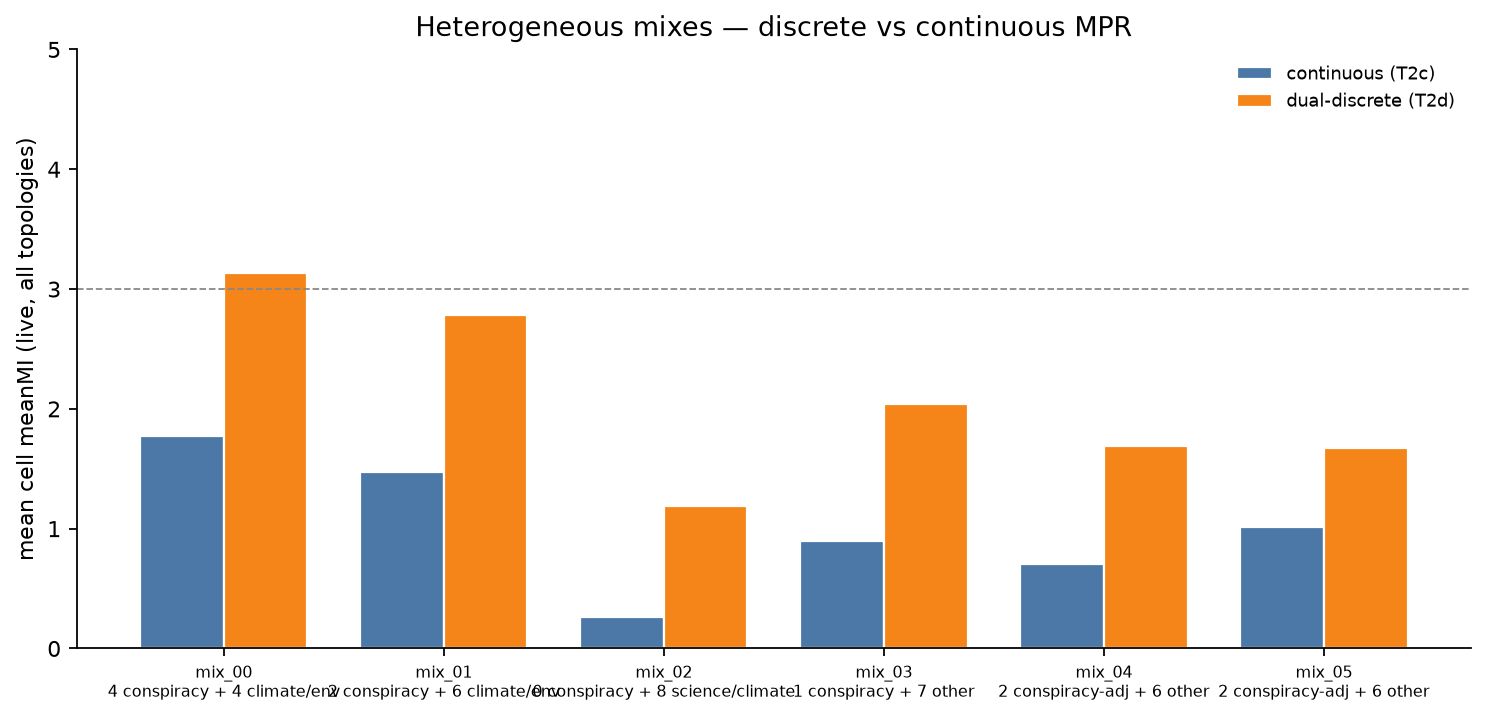
\includegraphics[width=\textwidth]{figures/fig04_mix_mpr_bars.png}
\caption{Heterogeneous mixes: live-cell mean \texttt{meanMI} collapsed across eight topologies, discrete versus continuous.
$N=1$, 48 cells per mix per mode before hatching.
Source: \texttt{fig04\_mix\_mpr\_bars.png}.}
\label{fig:mix}
\end{figure}

\begin{figure}[t]
\centering
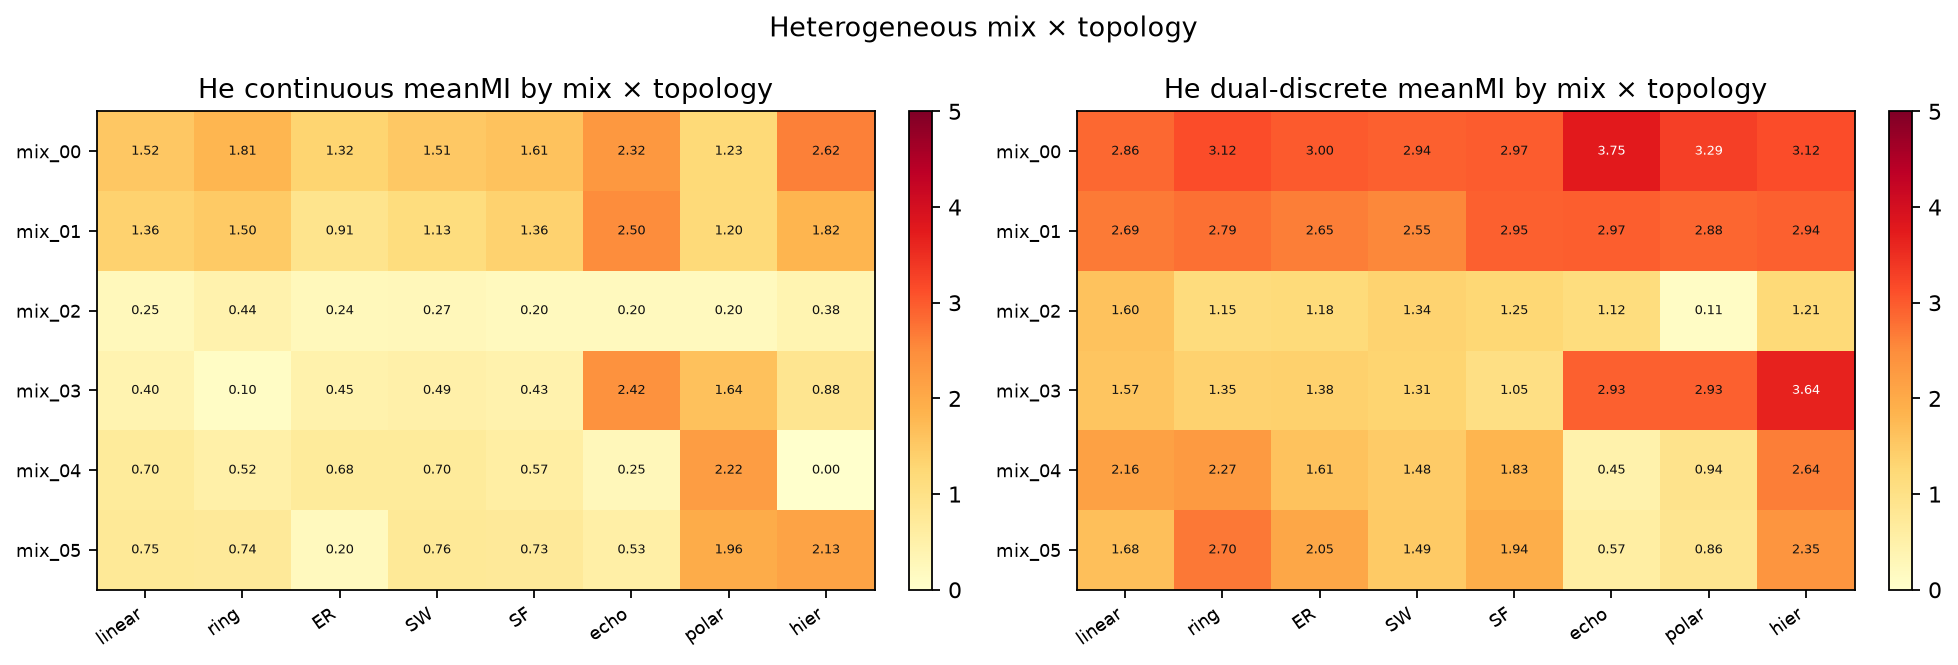
\includegraphics[width=\textwidth]{figures/fig07_mix_topology_heatmaps.png}
\caption{Heterogeneous mix $\times$ topology heatmaps of live-cell \texttt{meanMI}.
Left: continuous.
Right: dual-discrete.
$N=1$.
Source: \texttt{fig07\_mix\_topology\_heatmaps.png}.}
\label{fig:heatMT}
\end{figure}

\begin{table}[t]
\centering
\caption{Heterogeneous mixes collapsed across topologies.}
\label{tab:mix}
\begin{tabular}{llrrrr}
\toprule
Mix & Composition & Disc.\ \MPR{} & Cont.\ \MPR{} & \kstar{} dual & \kstar{} cont. \\
\midrule
mix\_00 & 4 conspiracy + 4 climate/env. & 3.1321 & 1.7712 & 57.5\% & 12.8\% \\
mix\_01 & 2 conspiracy + 6 climate/env. & 2.7795 & 1.4770 & 58.5\% & 9.8\% \\
mix\_02 & 0 conspiracy + 8 science/climate & 1.1882 & 0.2645 & 0.0\% & 0.0\% \\
mix\_03 & 1 conspiracy + 7 other & 2.0410 & 0.8945 & 33.3\% & 10.3\% \\
mix\_04 & 2 conspiracy-adj.\ + 6 other & 1.6896 & 0.7021 & 20.5\% & 5.3\% \\
mix\_05 & 2 conspiracy-adj.\ + 6 other & 1.6713 & 1.0134 & 23.3\% & 7.5\% \\
\bottomrule
\end{tabular}
\end{table}

\section{Four comparison designs}
\label{sec:designs}

The previous paper organised empirical comparison around homogeneous versus heterogeneous identity, hop-limited trajectories, persona-conditioned heatmaps, and networked conditions \parencite{maurya2025simulating}.
The thesis protocol names four designs that this climate campaign can instantiate without reprinting crime-news cells.
Phase~2 reports those four designs on the live harvest.
Belief-correction injection (Phase~1 Experiment~B, $n\in\{1,3\}$) was not repeated here; Design~C below is therefore seed valence, which Phase~2 did sweep.

Each design is a contrast, not a significance test.
$N=1$ supplies point estimates only.

\subsection{Design A: linear-chain analogue}

Design~A repeats the CIKM topology idea --- a linear chain --- on the climate corpus \parencite{maurya2025simulating}.
Homogeneous chains assign one persona; heterogeneous chains cycle a mix.
The engine object is \texttt{linear\_chain} with eight nodes and drip seed \texttt{node\_0}.
The hop budget is eight, not CIKM~30.

\Cref{tab:topoH,tab:topoHe} already contain the chain rows.
H continuous chain \MPR{} is $0.9129$ ($n=62$ live of 72).
H dual-discrete chain \MPR{} is $1.6127$ ($n=68$).
He continuous chain \MPR{} is $0.8638$ ($n=32$ of 36).
He dual-discrete chain \MPR{} is $2.0852$ ($n=33$).

On the continuous instrument, the He chain sits slightly below the H chain ($0.8638$ versus $0.9129$).
On the discrete instrument, the He chain sits above the H chain ($2.0852$ versus $1.6127$).
The two instruments disagree on the CIKM-style ordering for this topology.
A climate-domain claim that \enquote{heterogeneous chains buffer} therefore fails already at the instrument split, before any article-wise majority test.
\texttt{mix\_02} inside the He collapse is the expert-inclusive mix that the CIKM analogue requires; the He chain mean still includes \texttt{mix\_00}.
Composition again dominates the label.

Design~A is eligible as a protocol (climate chains exist).
It is not a successful conceptual replication of the CIKM homo$>$hetero severity pattern under the criteria in the discovery notes: six articles rather than $\ge 10$, $N=1$, \texttt{gpt-4o-mini} only, and mode disagreement on the collapsed chain.

\subsection{Design B: networked topology and \texorpdfstring{\kstar{}}{k*}}

Design~B is the networked expansion: eight generators $\times$ identity $\times$ two instruments, with irreversible \kstar{} as the firestorm clock.
Section~\ref{sec:topology} is the full table.
The design question is whether hubs, chambers, or hierarchy move live \MPR{} and \kstar{} relative to a short path or an ER null, holding the seed set fixed.

No generator dominates both instruments and both arms.
Scale-free is highest on H continuous and mid-pack on He continuous.
Echo chamber is highest on H dual-discrete and mid-pack on He dual-discrete.
Hierarchical He is highest on both He instruments and also among the deadliest cells.
ER He is lowest on continuous \MPR{} ($0.6593$) with continuous \kstar{} $0.0\%$ on 29 live cells, yet dual-discrete ER He remains $2.0412$ with \kstar{} $27.6\%$.

Design~B therefore supports only a weak descriptive statement.
Topology rank is mode-dependent and arm-dependent.
Hub generators do not uniquely produce textbook \kstar{} in this $N=1$ eight-tick window.
The statement \enquote{scale-free causes firestorms} is not licensed.

\subsection{Design C: seed valence}

Design~C holds topology and mix in the collapse and contrasts articles.
\textcite{pfeffer2014firestorms} describe firestorm messages as affectively charged; they do not number a factor called valence.
The campaign treats article wording as the valence knob: calm SCoPEx measurement text versus high-arousal chemtrails--Gates text, plus four further climate items.

\Cref{tab:articles} reports live-cell means by article, arm, and instrument.
On both arms, \texttt{climate\_consensus} and \texttt{chemtrails\_gates\_2018\_2021} sit at the high end.
\texttt{polar\_bears} sits at the low end, especially on continuous H ($0.0166$) and He ($0.0415$).
\texttt{sai\_geoengineering} is low on continuous and only moderate on discrete.
\texttt{scopex\_2017} is not uniformly the calmest cell: H discrete $1.5390$ exceeds H discrete polar bears ($1.0399$), while H continuous SCoPEx ($0.7321$) far exceeds H continuous polar bears.

The predicted H1 direction (chemtrails $>$ SCoPEx on the same cells) holds in this collapse for both arms and both instruments.
Chemtrails H continuous $1.3585$ exceeds SCoPEx H continuous $0.7321$; chemtrails H discrete $2.1383$ exceeds SCoPEx H discrete $1.5390$.
The same sign appears on He.
The contrast still confounds topic, frame, and prior conspiracy fit.
It is compatible with a valence reading.
It is not a test that isolated emotional charge.

\begin{table}[t]
\centering
\caption{Article (valence) collapse.
Articles are a factor, not statistical replicates.
$N=1$.}
\label{tab:articles}
\begin{tabular}{lrrrr}
\toprule
Article & H discrete & H continuous & He discrete & He continuous \\
\midrule
scopex\_2017 & 1.5390 & 0.7321 & 2.3718 & 0.7694 \\
chemtrails\_gates\_2018\_2021 & 2.1383 & 1.3585 & 2.3885 & 1.7852 \\
sai\_geoengineering & 1.3576 & 0.1946 & 1.1160 & 0.1523 \\
paris\_agreement & 1.7321 & 1.3334 & 2.4591 & 1.6821 \\
climate\_consensus & 2.2610 & 1.5721 & 2.8991 & 1.8896 \\
polar\_bears & 1.0399 & 0.0166 & 1.1444 & 0.0415 \\
\bottomrule
\end{tabular}
\end{table}

\subsection{Design D: closed-group wiring}

Design~D asks whether echo-chamber and polarised generators concentrate distortion relative to open graphs (ER, small-world, chain) on the same identity mix.
Pfeffer factor~3 (network clusters) and parts of factor~4 (unrestrained flow) and factor~5 (homophily) are the 2014 sources for this remapping \parencite{pfeffer2014firestorms}.
Phase~1's extra echo cell died at tick~1 with zero LLM calls.
Phase~2 completed echo-chamber and polarised cells on both arms; those cells can be described.
They still cannot be sold as emergent echo, because the generators \emph{input} chambers.

On homogeneous continuous cells, echo ($0.8233$) and polarised ($0.8356$) sit below scale-free ($0.9205$) and even below the linear chain ($0.9129$).
Closed wiring does not raise H continuous \MPR{} in this harvest.
On homogeneous dual-discrete cells, echo is the highest generator ($1.7984$).
The instrument split again forbids a single echo claim.

On heterogeneous continuous cells, echo ($1.3775$), polarised ($1.4137$), and hierarchical ($1.5242$) sit well above ER ($0.6593$) and the linear chain ($0.8638$).
Closed or tiered wiring coincides with higher He continuous \MPR{} here.
Polarised He is also 30.6\% dead on continuous, so the live mean is a selected subset.
He dual-discrete does not repeat the same ranking: hierarchical leads ($2.5934$), and polarised is lowest ($1.8830$) among the eight.

Design~D therefore yields a mode- and arm-conditional description.
He continuous cells on echo and polarised graphs scored higher than He continuous cells on ER in this $N=1$ draw.
H continuous cells did not.
The Phase~1 dead echo cell is not recycled as a negative finding; the Phase~2 echo cells are live enough to describe and still too weakly replicated to confirm H5.

\section{C5: cell pooling is not a super-graph}
\label{sec:pooled}

C5 concatenates live article-cells across the eight 8-node topologies.
That operation is a table union.
It is not a physical 64-node graph, and it is not the 63-node D-net custom topology.
\Cref{fig:c5pool} shows the four instrument-by-arm headlines on the concatenated set.

\begin{figure}[t]
\centering
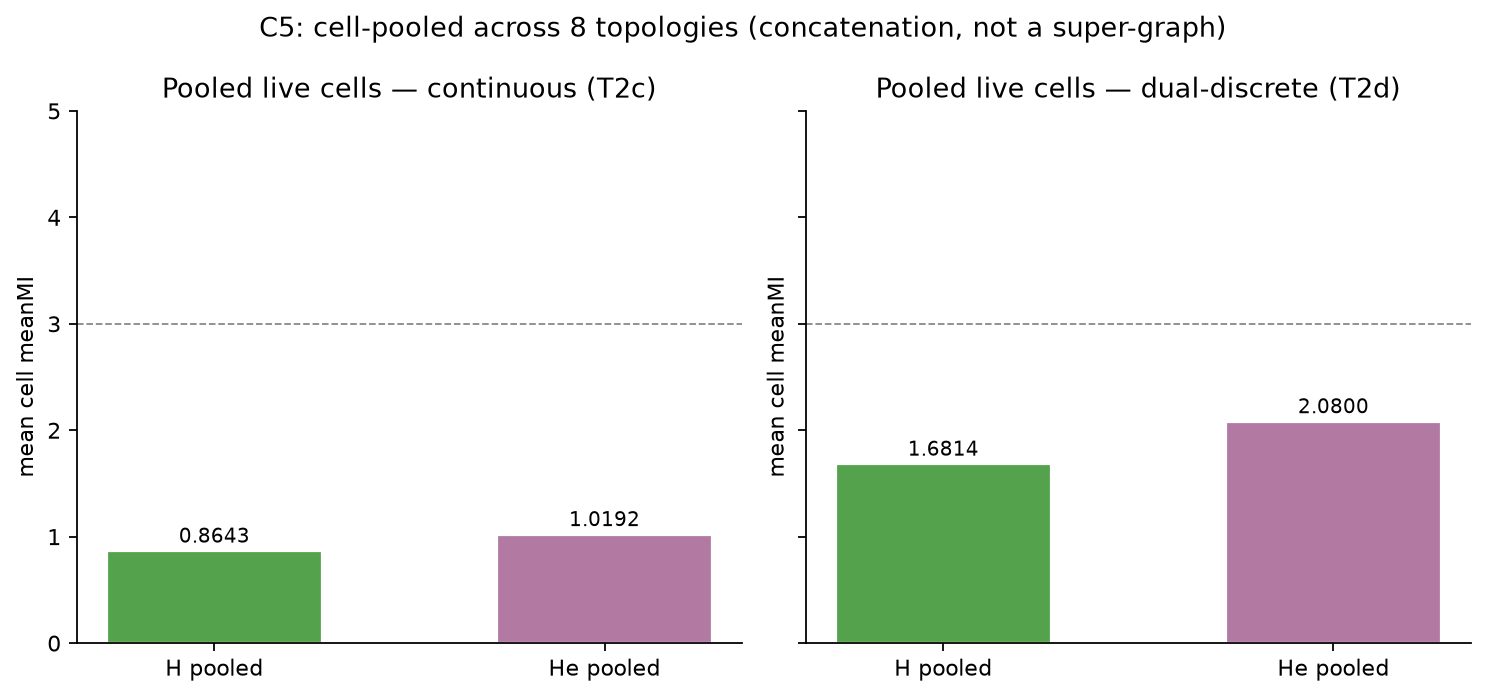
\includegraphics[width=\textwidth]{figures/fig06_c5_pooled_h_vs_he.png}
\caption[C5 cell-pooled H vs He]{C5: cell-pooled H versus He on concatenated live rows.
Pooling is not a super-graph.
$N=1$.
Source: \texttt{fig06\_c5\_pooled\_h\_vs\_he.png}.}
\label{fig:c5pool}
\end{figure}

On the concatenated set, He still exceeds H on both instruments (continuous $\Delta=0.1549$; dual-discrete $\Delta=0.3986$).
Topology-equal weighting does not flip the sign (\Cref{tab:c5w,tab:c5pool}).
The sign is compatible with conspiracy composition, not with a buffering law.

T2c family mean \MI{} on pooled H cells is conspiracy $2.2194$, climate action $0.1729$, science/environment $0.1118$.
T2d family means are conspiracy $3.1691$, climate action $1.0488$, science/environment $0.8687$.
On pooled He cells, \texttt{mix\_00} (four conspiracy) is T2c $1.7712$ versus \texttt{mix\_02} (zero conspiracy) $0.2645$; T2d \texttt{mix\_00} is $3.1321$ versus \texttt{mix\_02} $1.1882$.
Restricting H to the conspiracy family reverses the naive H/He story: conspiracy H sits well above overall He.
\Cref{fig:c5comp} records that composition split.

\begin{figure}[t]
\centering
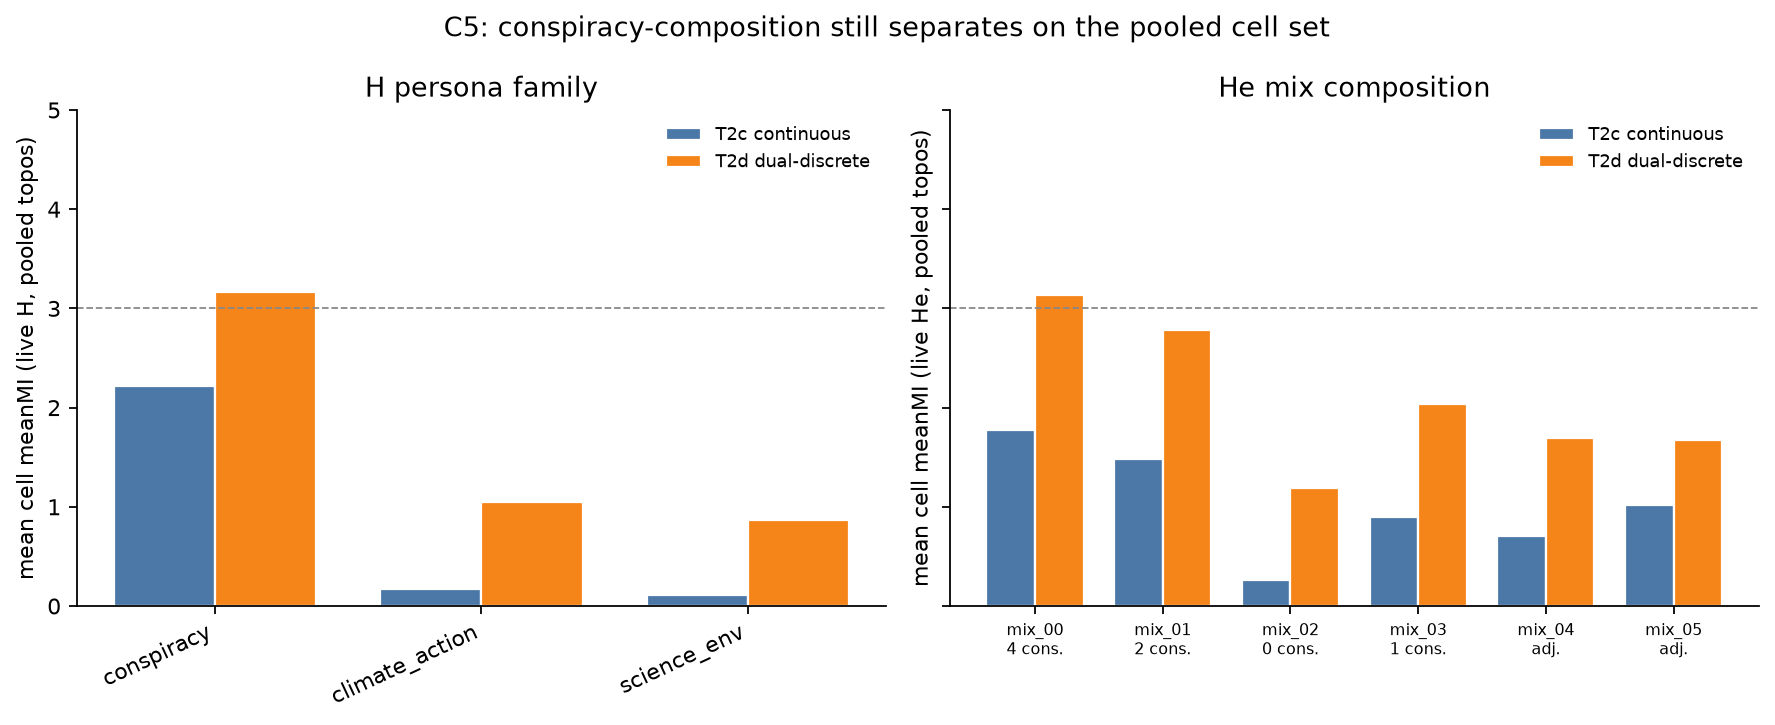
\includegraphics[width=\textwidth]{figures/fig07_c5_conspiracy_composition.png}
\caption[C5 conspiracy composition]{C5: family means on pooled H cells and mix means on pooled He cells.
Conspiracy remains the high group on both instruments.
$N=1$.
Source: \texttt{fig07\_c5\_conspiracy\_composition.png}.}
\label{fig:c5comp}
\end{figure}

\begin{table}[t]
\centering
\caption[C5 concatenated live-cell pools]{C5 concatenated live-cell pools.
These rows are table unions, not a 64-node graph and not D-net.}
\label{tab:c5pool}
\scriptsize
\begin{tabular}{lrrrr}
\toprule
Pool & $n$ live & meanMI & meanNodeMPR & \kstar{} rate \\
\midrule
T2c\_H all topologies & 480 & 0.8643 & 0.8630 & 14.2\% \\
T2c\_He all topologies & 238 & 1.0192 & 1.0140 & 7.6\% \\
T2d\_H all topologies & 478 & 1.6814 & 1.6839 & 20.1\% \\
T2d\_He all topologies & 240 & 2.0800 & 2.0737 & 32.1\% \\
T2c\_H conspiracy family & 168 & 2.2194 & 2.2145 & 40.5\% \\
T2c\_H science/env.\ family & 195 & 0.1118 & 0.1130 & 0.0\% \\
T2c\_H climate-action family & 117 & 0.1729 & 0.1724 & 0.0\% \\
T2d\_H conspiracy family & 159 & 3.1691 & 3.1799 & 59.7\% \\
T2c\_He mix\_00/\_01 (conspiracy-heavy) & 80 & 1.6204 & 1.5921 & 11.2\% \\
T2c\_He mix\_02 (conspiracy-free) & 41 & 0.2645 & 0.2648 & 0.0\% \\
\bottomrule
\end{tabular}
\end{table}

\begin{table}[t]
\centering
\caption[C5 cell-pooled versus topology-equal]{C5: cell-pooled versus topology-equal H/He means.
Neither column is a super-graph.}
\label{tab:c5w}
\begin{tabular}{lrrrrrr}
\toprule
Contrast & Pooled H & Pooled He & $\Delta$ & Topo-eq.\ H & Topo-eq.\ He & $\Delta$ \\
\midrule
T2c H vs He & 0.8643 & 1.0192 & 0.1549 & 0.8630 & 1.0356 & 0.1725 \\
T2d H vs He & 1.6814 & 2.0800 & 0.3986 & 1.6832 & 2.0806 & 0.3974 \\
\bottomrule
\end{tabular}
\end{table}

\paragraph{Invalid extra pools.}
Averaging discrete with continuous H still has no auditor ($(0.8643+1.6814)/2=1.2729$).
Averaging H with He inside one instrument still hides composition.
D-net rows are not concatenated into \Cref{tab:c5w}.
Section~\ref{sec:dnet} treats the 63-node custom graph as a separate object.

\section{D-net, Pfeffer observables, and Debnath}
\label{sec:dnet}

The D-net arm imports a reconstructed graph and runs the same two scoring modes on homogeneous conspiracy and mixed identities.
The empirical file is \path{thesisExperiment/data/derived/debnath_hashtag_cascade.json}.
Kind: hashtag co-occurrence.
\texttt{notARetweetCascade: true}.
Nodes are users keyed by published hashtags (63 nodes, 228 directed edges, 171 unique undirected pairs).
Edges reuse a \texttt{retweets[]} container only as a directed-edge slot.
The graph is not a hydrated retweet cascade.
The comparable simulated object is this 63-node custom topology, not the eight 8-node T2 generators.

Hydration of Debnath's tweet identifiers failed.
Mendeley \texttt{10.17632/546hsym93p.1} is an identifier dump, not tweet text \parencite{debnath2023dataset}.
814,924 tweets were not hydrated.
Belief profiles remain theory-faithful reductions, not skip-gram/HDBSCAN centroids \parencite{debnath2023conspiracy,geoeng2023codes}.
Debnath reports no empirical $0$--$5$ \MPR{}.
Simulated auditor \MI{} is therefore not Twitter \MI{} \parencite{ruths2014social}.

Mapping from hashtag cluster to Debnath type was already in the Dnet configs.
No new LLM runs were added for this note.
Empirical cluster identity is conspiracy 28, climate action 19, environmental 14, expert 2.
Mixed Dnet preserves that type mix (conspiracy share $0.444$).
Homogeneous Dnet overwrites every seat to \texttt{conspiracy\_believer} (share $1.0$).
Exact persona-identifier match reconstruct$\leftrightarrow$mixed is 56 of 63; seven seats stay in the same Debnath type on a coarser library id.
Averaged compare \texttt{conspiracyShare=0.722} is H+He pooled and is not a third mix.

\subsection{C5 D-net auditor scores (not pooled into T2)}

\Cref{fig:c5dnet} and \Cref{tab:dnetmpr} list LLM-as-judge headlines on the custom graph.
On D-net, homogeneous conspiracy exceeds mixed identity on both instruments and both seeds.
Continuous SCoPEx: H $1.7349$ versus He $0.9983$.
Continuous chemtrails: H $3.3378$ versus He $2.5068$.
Dual-discrete SCoPEx: H $4.2537$ versus He $2.6880$.
Dual-discrete chemtrails: H $3.7303$ versus He $1.5297$.

That ordering matches composition (D-net H is conspiracy-only).
It does not match the naive eight-topology collapsed He$>$H, which mixed scientists into H.
The H/He label does not travel unchanged onto the 63-node graph.
Dual versus continuous still must not be averaged.
Chemtrails raises continuous \MI{} versus SCoPEx on the same graph; the dual headline does not preserve that article order on He.

\begin{figure}[t]
\centering
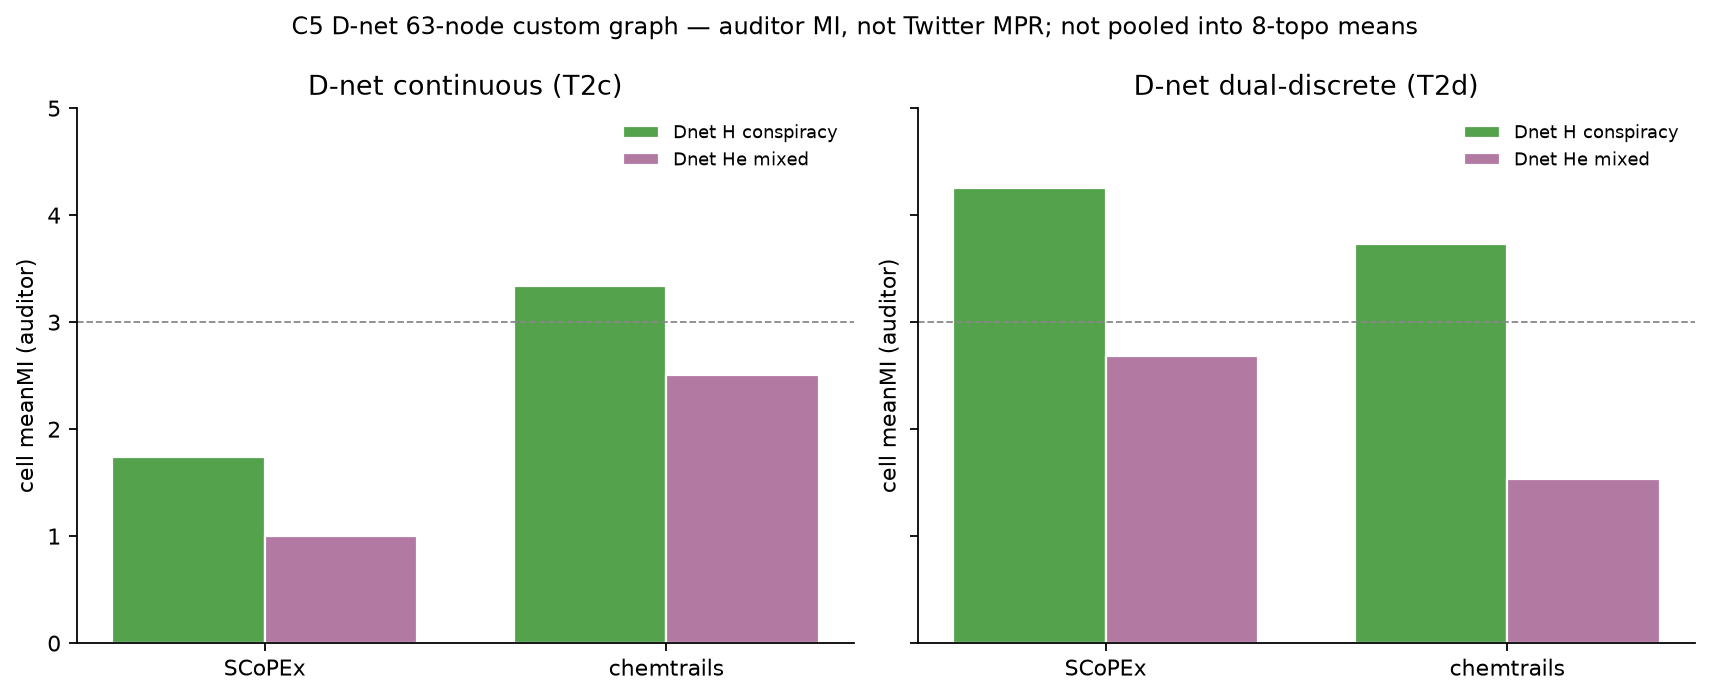
\includegraphics[width=\textwidth]{figures/fig08_c5_dnet.png}
\caption[C5 D-net auditor MI]{C5: D-net 63-node auditor \MI{} by mix, article, and instrument.
Not Twitter \MPR{}.
Not concatenated into the eight T2 topologies.
$N=1$.
Source: \texttt{fig08\_c5\_dnet.png}.}
\label{fig:c5dnet}
\end{figure}

\begin{table}[t]
\centering
\caption{D-net auditor headlines on the hashtag co-occurrence graph.
Sidecar continuous on dual runs is not the T2c headline.}
\label{tab:dnetmpr}
\small
\begin{tabular}{llllr}
\toprule
Run & Article & Mode & Disc.\ \MPR{} & Cont.\ \MPR{} \\
\midrule
Dnet\_c\_H\_conspiracy & SCoPEx & continuous & --- & 1.7349 \\
Dnet\_c\_H\_conspiracy & chemtrails--Gates & continuous & --- & 3.3378 \\
Dnet\_c\_He\_mixed & SCoPEx & continuous & --- & 0.9983 \\
Dnet\_c\_He\_mixed & chemtrails--Gates & continuous & --- & 2.5068 \\
Dnet\_d\_H\_conspiracy & SCoPEx & dual-disc. & 4.2537 & sidecar 2.2495 \\
Dnet\_d\_H\_conspiracy & chemtrails--Gates & dual-disc. & 3.7303 & sidecar 3.1251 \\
Dnet\_d\_He\_mixed & SCoPEx & dual-disc. & 2.6880 & sidecar 1.1302 \\
Dnet\_d\_He\_mixed & chemtrails--Gates & dual-disc. & 1.5297 & sidecar 1.1497 \\
\bottomrule
\end{tabular}
\end{table}

\subsection{Structural comparison}

\Cref{fig:dnet} and \Cref{tab:struct} compare empirical hashtag-graph cascade-shape metrics with the mean of 16 simulated D-net cascades.
Structural similarity (share of compared metrics within a 30\% band) is $0.6885$: breadth matches, depth and structural virality \parencite{goel2016virality} do not.
Kolmogorov--Smirnov tests use $n_{\mathrm{real}}=1$ and $n_{\mathrm{sim}}=16$ and are underpowered.
DTFS $=0.2754$ with \texttt{isValidated=false} (threshold $0.70$).
That table is cascade shape, not a Pfeffer factor.

Empirical transitivity is $0.315$; mean local clustering is $0.515$; the chemtrails hub has 33 unique neighbours.
D-net copies that graph; it does not grow clusters.
On 171 unweighted unique-undirected pairs, the binary conspiracy cut has Newman--Girvan $Q=0.4297$ under mixed labels.
The homogeneous assignment is one community and therefore has $Q=0$.
The six assigned graph clusters instead have $Q=0.5489$; modularity of a label partition is not a clustering coefficient.

\begin{figure}[t]
\centering
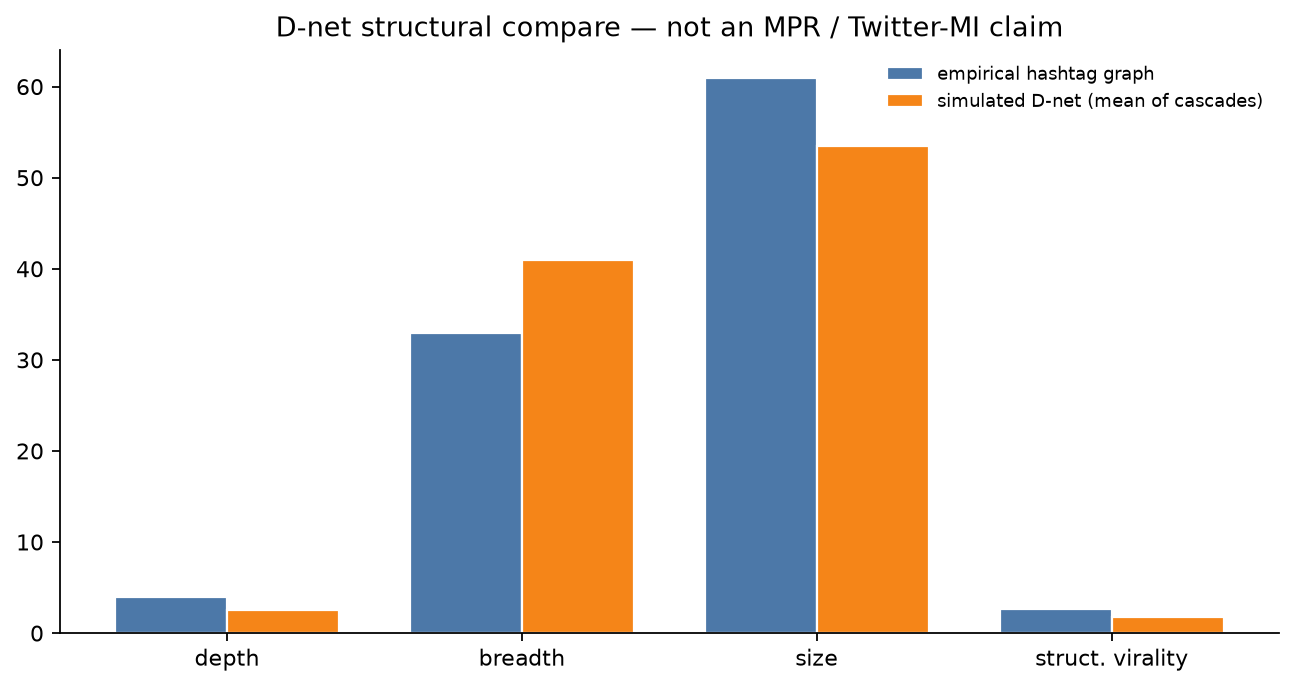
\includegraphics[width=0.88\textwidth]{figures/fig09_dnet_structural.png}
\caption[D-net structural compare]{Empirical hashtag-graph metrics versus mean simulated D-net metrics (16 cascades).
This is a structural comparison, not an \MPR{} or Twitter-\MI{} claim.
Source: \texttt{fig09\_dnet\_structural.png}.}
\label{fig:dnet}
\end{figure}

\begin{table}[t]
\centering
\caption{D-net structural metrics.
Match $=$ within a 30\% band of the empirical value.
KS/JS: $n_{\mathrm{real}}=1$, underpowered.}
\label{tab:struct}
\small
\begin{tabular}{lrrll}
\toprule
Metric & Emp. & Sim.\ mean & Match (30\%) & Note \\
\midrule
depth & 4 & 2.5625 & no & longest path from root \\
breadth & 33 & 40.9375 & yes & max nodes at one level \\
size & 61 & 53.5 & --- & informational \\
struct.\ virality & 2.7 & 1.7963 & no & \textcite{goel2016virality} \\
speed & n/a emp. & 8 ticks & --- & do not convert ticks to hours \\
mean \MI{} & no emp.\ \MPR{} & 2.5529 & do not equate & auditor only \\
\bottomrule
\end{tabular}
\end{table}

\subsection{Pfeffer 2014: seven factors, then a remapping}

\textcite{pfeffer2014firestorms} list seven interrelated factors in the Outlook section:
\begin{enumerate}[nosep]
\item speed and volume of communication;
\item binary choices (like/share/retweet as either--or);
\item network clusters;
\item unrestrained information flow;
\item lack of diversity;
\item cross-media dynamics;
\item network-triggered decision processes.
\end{enumerate}
That list is the primary theory.
The thesis six-knob vocabulary is a computational remapping, not a restatement of the 2014 paper.
\Cref{tab:pfeffer} splits homogeneous from mixed simulation so that homophily $1.0$ is not pooled as a third mix.

Identity-edge homophily on the empirical graph is $0.873$ (BP-family $0.838$).
Mixed Dnet reproduces block echo (identity homophily $0.838$).
Homogeneous Dnet reports homophily $1.0$ because identity was erased.
The earlier harvest row that averaged H+He into \texttt{edgeHomophily=1} is a homogeneous artefact.

Binary choices (Outlook \#2) have no engine row.
Scored actions are ternary, with reinterpret about $0.46$--$0.53$.
That pattern is the opposite of limited like/share interaction.
Cross-media (Outlook \#6) remains held: no broadcast agent.
Surprise is held drip from \texttt{user\_chemtrails\_hub}.
Temporal series are not available empirically; the sim clock is eight ticks, and 61 of 63 nodes are reached in all four primary cells.
Outlook \#4 (hundreds to thousands of weak ties) is not this 63-node hub of degree 33.

\begin{table}[t]
\centering
\caption{Pfeffer observables on the Debnath hashtag fallback versus simulated D-net, H and He split.
Empirical valence is a toxicity/hashtag proxy, not \MPR{}.
Simulated \MI{} is an auditor score, not Twitter \MI{}.}
\label{tab:pfeffer}
\scriptsize
\begin{tabular}{>{\raggedright\arraybackslash}p{0.14\textwidth}
                >{\raggedright\arraybackslash}p{0.20\textwidth}
                >{\raggedright\arraybackslash}p{0.28\textwidth}
                >{\raggedright\arraybackslash}p{0.26\textwidth}}
\toprule
Observable & Pfeffer 2014 map & Empirical & Simulated (split) \\
\midrule
valence & affective character (definition), not an Outlook number & hashtag prior $0.1097$; paper toxicity mean $0.17$ & auditor \MI{}; chemtrails $>$ SCoPEx on continuous H and He \\
surprise & \#1 speed/volume (shock vs drip) & paper SCoPEx spike; not reconstructed & held drip from chemtrails hub \\
identity & \#5 lack of diversity & conspiracy share $0.444$ & H $1.0$; He $0.444$; do not pool to $0.722$ \\
clustering & \#3 network clusters & transitivity $0.315$; local $0.515$; graph-cluster $Q=0.5489$ & same topology; conspiracy-cut $Q=0.4297$ mixed, one-community $Q=0$ \\
echo & \#3 + \#4 + parts of \#5 & identity homophily $0.873$ & He $0.838$; H $1.0$ by construction \\
temporal & \#1 / \#7 & not available (no tweet clock) & 8 ticks; 61/63 nodes reached \\
cross-media & \#6 & held & held (no engine knob) \\
binary choices & \#2 (no thesis knob) & no like/retweet actions & ternary rewrite, not Schelling binary \\
\bottomrule
\end{tabular}
\end{table}

The table is an honesty ledger, not a seven-factor confirmation.
Clustering here is an empirical-structure result copied into D-net.
Echo is label-dependent.
Surprise, temporal acceleration, and cross-media were held or missing empirically.

\section{Limitations}
\label{sec:limits}

The harvest itself marks this campaign as not thesis-grade (\texttt{thesisGrade: false}).
The following limits are part of the result, not an appendix apology.

\paragraph{$N=1$.}
One graph seed ($42$), one run per config.
No error bars, no topology significance tests, no permutation tests.
Events on the same node share inbox and trust state; nodes share a graph.
Treating scored events as i.i.d.\ replicates would inflate precision.

\paragraph{Eight hops are not CIKM 30.}
The hop/tick budget is a logged cost compression versus the CIKM chain length of 30 \parencite{maurya2025simulating}.
It is not Debnath's hop protocol and not an empirical firestorm duration.
\kstar{} irreversibility is right-censored at eight ticks.

\paragraph{Debnath's eight is a skip-gram window.}
\textcite{debnath2023conspiracy} define a context window of eight \emph{words} for skip-gram embeddings.
That hyperparameter is unrelated to this campaign's eight hops.

\paragraph{Hatched dead cells: 290.}
Dead cells are kept.
They are not zeros and they are not mix immunity.
Live-only means drop those cells and therefore describe surviving cascades.
Hierarchical and some polarised He slices are particularly incomplete.

\paragraph{Two instruments.}
Dual-discrete headline $\neq$ continuous headline.
Dual gap $\neq$ \MPR{}.
Section~\ref{sec:pooled} lists the pooled scalars that must not re-enter the abstract.

\paragraph{Hashtag graph, not a retweet cascade.}
The Debnath reconstruct is a hashtag co-occurrence fallback.
814k tweet identifiers were not hydrated \parencite{debnath2023dataset}.
BPs are theory-faithful reductions, not HDBSCAN centroids.
No empirical \MPR{} exists on Debnath, so simulated \MI{} cannot \enquote{match Twitter misinformation}.

\paragraph{KS/JS with $n_{\mathrm{real}}=1$.}
Distributional tests cannot support a digital-twin claim.
DTFS failed the $0.70$ threshold ($0.2754$).

\paragraph{Pfeffer 2014 has seven factors.}
The thesis six-knob list is a remapping \parencite{pfeffer2014firestorms}.
Cross-media is held (no engine knob).
Surprise is held as drip.
Binary like/share is not the engine's ternary action set.

\paragraph{Role-play is not a field community.}
\texttt{gpt-4o-mini} system prompts can produce prompt-faithful conspiracy language \parencite{park2023generative}.
High conspiracy \MPR{} is compatible with obedience to those prompts.
It is not, by itself, evidence of stubborn belief or of chemtrails communities in the wild.
False news online does travel farther than true news in observational cascades \parencite{vosoughi2018false}; this simulator does not re-estimate that fact.

\paragraph{Auditor as truth.}
Five author-written QA items define \MI{}.
A different key would move the numbers.
Ground truth is the curated scientific record in the article pack, not a moral ranking of personas.
Human-eval templates exist in run directories and were not completed as an IRB study.

\paragraph{Phase~1 is a different campaign.}
The discrete $12\times 12$ chain tables under \path{thesisExperiment/results/tables/} are not spliced into these headlines.
Fact-check injection (Experiment~B) and the distortion keyword heuristic (Experiment~C) belong to that earlier drop-in set unless a later pass re-runs them under \texttt{runs\_phase2/}.

\paragraph{Correction literature is out of scope here.}
Continued-influence and debiasing results \parencite{lewandowsky2012misinformation} motivated Phase~1 Experiment~B.
Phase~2 does not estimate recovery.

\section{Chapter conclusion}
\label{sec:conclusion}

Phase~2 completed the eight-topology $\times$ H/He $\times$ dual/continuous grid ($1{,}728$ cells, $0$ missing) plus four D-net configs.
The harvest is a real-\texttt{gpt-4o-mini} $N=1$ pilot with \texttt{thesisGrade=false}.

Four headlines stand, and they are not interchangeable.
Homogeneous continuous \MPR{} is $0.8608$ ($n=482$ live).
Homogeneous dual-discrete \MPR{} is $1.6814$ ($n=478$).
Heterogeneous continuous \MPR{} is $1.0192$ ($n=238$).
Heterogeneous dual-discrete \MPR{} is $2.0800$ ($n=240$).
Dual-discrete sits higher than continuous on every topology.
That is a scoring-mode effect.

Collapsed He exceeds collapsed H on both instruments.
Composition explains the sign: conspiracy personas and conspiracy-heavy mixes score high; science personas and \texttt{mix\_02} score low.
The H/He label is not a buffering law.

Topology rank depends on instrument and arm.
No generator is \enquote{the firestorm topology} in this draw.
Echo and polarised He continuous cells scored higher than ER He continuous cells; H continuous cells did not repeat that pattern.
Hierarchical He leads both He instruments and is heavily hatched.

Design~A (climate chains) is protocol-complete and inconclusive as a CIKM conceptual replication: the two instruments disagree on the collapsed chain ordering, and six articles with $N=1$ do not meet the pre-registered success bar.
Design~B (networked \kstar{}) shows mode-dependent ranks and weak irreversibility on an eight-tick clock.
Design~C (valence) shows chemtrails $>$ SCoPEx in the article collapse, still confounded with topic and prior fit.
Design~D (closed-group wiring) is describable because Phase~2 echo cells lived; it does not confirm emergent echo.

The D-net comparison is structural.
Breadth lies within a 30\% band of the hashtag graph; depth and structural virality do not.
KS tests with one empirical graph are underpowered.
DTFS fails.
Simulated \MI{} is not Twitter \MPR{}.
Pfeffer, Zorbach and Carley list seven Outlook factors; this campaign remaps six knobs and holds cross-media.

What an examiner can accept is therefore narrow.
The engine produces non-zero, persona-sensitive auditor scores on climate seeds.
Conspiracy-conditioned nodes sit far above scientist-conditioned nodes on both instruments in this $N=1$ harvest.
Discrete and continuous campaigns must be reported as two leagues.
Everything else --- topology winners, hetero buffering, Twitter matching, seven-factor confirmation --- remains outside what these cells can carry.


\printbibliography[title={References}]

\end{document}
